\begin{frame}
	\myheading{Module 5.4 : Momentum based Gradient Descent}
\end{frame}

\begin{frame}
	\begin{overlayarea}{\textwidth}{\textheight}
		\begin{block}{Some observations about gradient descent}
			\begin{itemize}\justifying
				\item<1-> It takes a lot of time to navigate regions having a gentle slope
				\item<2-> This is because the gradient in these regions is very small
				\item<3-> Can we do something better ?
				\item<4-> Yes, let's take a look at `Momentum based gradient descent'
			\end{itemize}
		\end{block}
	\end{overlayarea}
\end{frame}

%\subsection{Momentum based gradient descent}
\begin{frame}
	\begin{overlayarea}{\textwidth}{\textheight}
		\begin{block}{Intuition}
			\begin{itemize}\justifying
				\item<1-> If I am repeatedly being asked to move in the same direction then I should probably gain some confidence and start taking bigger steps in that direction
				\item<2-> Just as a ball gains momentum while rolling down a slope
			\end{itemize}
		\end{block}
		
		\only<3->{
			\begin{block}{Update rule for momentum based gradient descent}
				\begin{align*}
					update_{t} & = \gamma\cdot update_{t-1} + \eta \nabla w_{t} \\
					w_{t+1}    & = w_{t} - update_{t}                           
				\end{align*}
				
				\begin{itemize}\justifying
					\item<4-> In addition to the current update, also look at the history of updates.
				\end{itemize}
			\end{block}
		}
	\end{overlayarea}
\end{frame}

\begin{frame}
	\begin{overlayarea}{\textwidth}{\textheight}
		\begin{align*}
			update_{t} & = \gamma\cdot update_{t-1} + \eta \nabla w_{t} \\
			w_{t+1}    & = w_{t} - update_{t}                           
		\end{align*}
		
		\vspace{0.1in}
		\begin{align*}
			\onslide<1->{update_{0} & = 0                                                                                                                                                                     \\}
			\onslide<2->{update_{1} & = \gamma\cdot update_{0} + \eta \nabla w_{1} = \eta \nabla w_{1}                                                                                                        \\}
			\onslide<3->{update_{2} & = \gamma\cdot update_{1} + \eta \nabla w_{2} = \gamma\cdot \eta \nabla w_{1} + \eta \nabla w_{2}                                                                        \\}
			\onslide<4->{update_{3} & = \gamma\cdot update_{2} + \eta \nabla w_{3} = \gamma (\gamma \cdot \eta \nabla w_{1} + \eta \nabla w_{2}) + \eta \nabla w_{3}                                          \\}
			\onslide<5->{           & = \gamma\cdot update_{2} + \eta \nabla w_{3} = \gamma^2 \cdot \eta \nabla w_{1} + \gamma \cdot \eta \nabla w_{2} + \eta \nabla w_{3}                                    \\}
			\onslide<6->{update_{4} & = \gamma\cdot update_{3} + \eta \nabla w_{4} = \gamma^3 \cdot \eta \nabla w_{1} + \gamma^2 \cdot \eta \nabla w_{2} + \gamma \cdot \eta \nabla w_{3} + \eta \nabla w_{4} \\}
			\onslide<7->{\vdots\\}
			\onslide<8->{update_{t} & = \gamma\cdot update_{t-1} + \eta \nabla w_{t} = \gamma^{t-1} \cdot \eta \nabla w_{1} + \gamma^{t-2} \cdot \eta \nabla w_{1} +  ... + \eta \nabla w_{t}                 \\}
		\end{align*}
		
		
	\end{overlayarea}
	
\end{frame}

\begin{frame}
	\begin{columns}
		\column{0.5\textwidth}
		\begin{overlayarea}{\textwidth}{\textheight}
			\vspace{-0.15in}
			\begin{figure}
				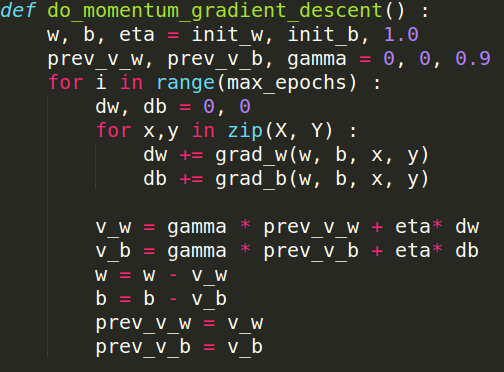
\includegraphics[scale=0.3]{images/module4/pseudo_code_mom_crop.png}
			\end{figure}
		\end{overlayarea}
		
		\column{0.5\textwidth}
		\begin{overlayarea}{\textwidth}{\textheight}
			\vspace{-0.15in}
			\foreach \n in {0,...,20} {%
				\begin{tikzpicture}
					\sbox0{\includegraphics[scale=0.4]{images/module4/mom1/2d_path\n.png}}% get width and height
					\only<\n>{\node[above right,inner sep=0pt] at (0,0)  {\usebox{0}}};
					\only<\n>{\node[red](w) at (0.5\wd0,0) {w}};
					\only<\n>{\node[red](b) at (0,0.67\ht0) {b}};
					\only<\n>{\draw[->, line width=0.2mm](w)--(0.6\wd0,0)};
					\only<\n>{\draw[->, line width=0.2mm](b)--(0,0.8\ht0)};
				\end{tikzpicture}
			}
			% \sbox0{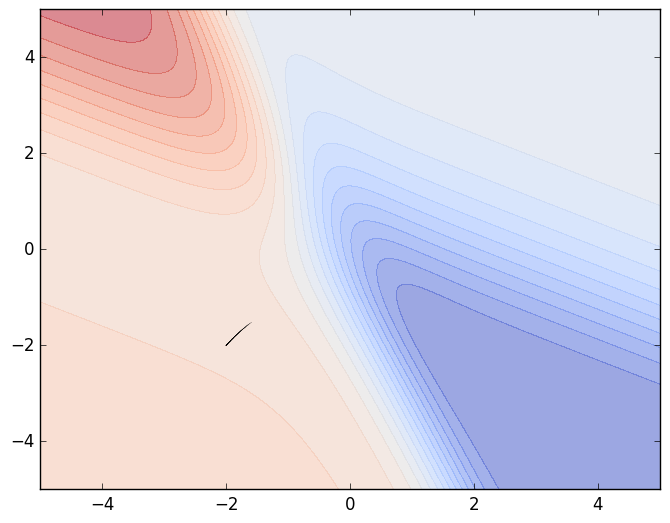
\includegraphics[scale=0.4]{images/module4/mom1/2d_path0.png}}% get width and height
		\end{overlayarea}
		
	\end{columns}
\end{frame}

\begin{frame}
	\begin{overlayarea}{\textwidth}{\textheight}
		\begin{block}{Some observations and questions}
			\begin{itemize}\justifying
				\item Even in the regions having gentle slopes, momentum based gradient descent is able to take large steps because the momentum carries it along
				      \item<2-> Is moving fast always good? Would there be a situation where momentum would cause us to run pass our goal?
				      \item<3-> Let us change our input data so that we end up with a different error surface and then see what happens ... 
			\end{itemize}
		\end{block}
	\end{overlayarea}
\end{frame}


\begin{frame}
	\begin{columns}
		\column{0.5\textwidth}
		\begin{overlayarea}{\textwidth}{\textheight}
			\begin{itemize}\justifying
				\item<2-> In this case, the error is high on either side of the minima valley
				\item<3-> Could momentum be detrimental in such cases... let's see....
			\end{itemize}
		\end{overlayarea}
		
		\column{0.5\textwidth}
		\begin{overlayarea}{\textwidth}{\textheight}
			\begin{figure}
				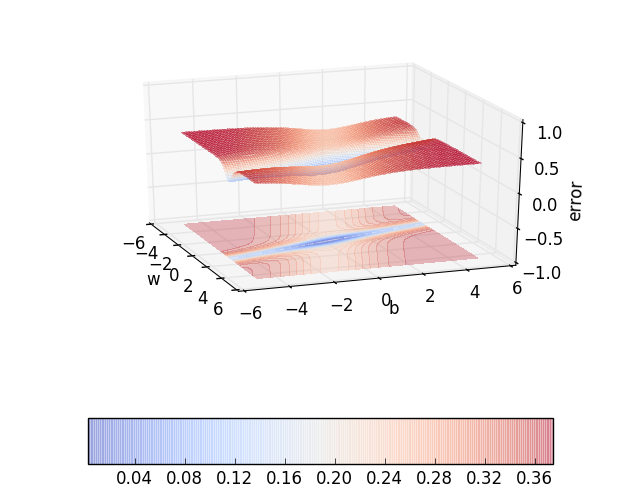
\includegraphics[scale=0.5]{images/module4/error_surface2.png}
			\end{figure}
		\end{overlayarea}
	\end{columns}
	
\end{frame}

\begin{frame}
	\begin{columns}
		\column{0.5\textwidth}
		\begin{overlayarea}{\textwidth}{\textheight}
			\begin{itemize}\justifying
				\item<37-> Momentum based gradient descent oscillates in and out of the minima valley as the momentum carries it out of the valley
				\item<38-> Takes a lot of \textit{u}-turns before finally converging 
				\item<39-> Despite these \textit{u}-turns it still converges faster than vanilla gradient descent
				\item<40-> After $100$ iterations momentum based method has reached an error of $0.00001$ whereas vanilla gradient descent is still stuck at an error of $0.36$ 
			\end{itemize}
		\end{overlayarea}
		
		\column{0.5\textwidth}
		\begin{overlayarea}{\textwidth}{\textheight}
			\begin{figure}
				\foreach \n in {0,...,40} {%
					\begin{tikzpicture}
						\sbox0{\includegraphics[scale=0.4]{images/module4/mom2/2d_path\n.png}}% get width and height
						\only<\n>{\node[above right,inner sep=0pt] at (0,0)  {\usebox{0}}};
						\only<\n>{\node[red](w) at (0.5\wd0,0.23\ht0) {w}};
						\only<\n>{\node[red](b) at (0,0.67\ht0) {b}};
						\only<\n>{\draw[->, line width=0.2mm](w)--(0.6\wd0,0.23\ht0)};
						\only<\n>{\draw[->, line width=0.2mm](b)--(0,0.8\ht0)};
					\end{tikzpicture}
				}
			\end{figure}
		\end{overlayarea}
	\end{columns}
	
\end{frame}

\begin{frame}
	\fontsize{16pt}{7.2}\selectfont
	\textit{Let's look at a 3d visualization and a different geometric perspective of the same thing...}
\end{frame}

\begin{frame}
	\begin{columns}
		\column{0.52\textwidth}
		\begin{overlayarea}{\textwidth}{\textheight}
			\begin{figure}
				\centering
				\foreach \n in {0,...,40} {%
					\includegraphics<\n>[scale=0.7]{images/module4/mom2/3d_path\n.png}
				}
			\end{figure}
		\end{overlayarea}
		
		\column{0.48\textwidth}
		\begin{overlayarea}{\textwidth}{\textheight}
			\begin{figure}
				\foreach \n in {0,...,40} {%
					\includegraphics<\n>[scale=0.4]{images/module4/mom2/sigmoid\n.png}
				}
			\end{figure}
		\end{overlayarea}
	\end{columns}
	
\end{frame}

